\documentclass[border=1.5pt]{standalone}
\usepackage{amsmath,amssymb}
\usepackage{tikz}
\usetikzlibrary{arrows.meta,calc,positioning,shapes,shapes.misc,shapes.geometric,backgrounds,fit,decorations.pathreplacing,quantikz2}
% Shared colors and styles for the XYZ^2 figures.
% Pauli types: bright tones for fills and bands, deep (800) shades of the same hues for labels.
% The label shades keep the hue of each Pauli, are well separated from each other (CIEDE2000 > 20)
% and have a contrast ratio of at least 2.9 on the coral cells and 4.5 on the sunflower cells.
\definecolor{PauliX}{HTML}{F97316}
\definecolor{PauliY}{HTML}{EC4899}
\definecolor{PauliZ}{HTML}{9333EA}
\definecolor{PauliXText}{HTML}{AC340B}
\definecolor{PauliYText}{HTML}{9D174D}
\definecolor{PauliZText}{HTML}{5B21B6}
% Generator classes: S0 (class B, even links, coral) and gauge (class A, odd links, sunflower)
\definecolor{Szero}{HTML}{F0435E}
\definecolor{SzeroText}{HTML}{BE123C}
\definecolor{Gauge}{HTML}{F59E0B}
\definecolor{GaugeText}{HTML}{B45309}
\colorlet{GaugeGray}{Gauge}
\definecolor{ClassB}{HTML}{FF8A99}
\definecolor{ClassA}{HTML}{FFD23F}
% Logical operators (X-bar violet, Z-bar crimson), errors, ink
\definecolor{LogicalZ}{HTML}{E11D48}
\definecolor{LogicalGold}{HTML}{7C3AED}
\definecolor{ErrRed}{HTML}{1C1917}
\definecolor{InkDark}{HTML}{292524}
\definecolor{InkSoft}{HTML}{57534E}
% Labels drawn on top of colored cells
\colorlet{CellText}{InkDark}
% Noise channels
\definecolor{ErrFlip}{HTML}{EF4444}
\definecolor{Idle}{HTML}{EC4899}
\definecolor{TwoQ}{HTML}{7C3AED}
% Protocol steps
\definecolor{StepPrep}{HTML}{F97316}
\definecolor{StepMeas}{HTML}{D946EF}
\definecolor{StepDec}{HTML}{7C3AED}
\definecolor{StepRec}{HTML}{DB2777}
\tikzset{
  qb/.style={circle, draw=InkDark, line width=0.6pt, fill=white,
             minimum size=4.2mm, inner sep=0pt, font=\scriptsize},
  qbsmall/.style={circle, draw=InkDark, line width=0.5pt, fill=white,
             minimum size=2.6mm, inner sep=0pt},
  hexedge/.style={line width=0.65pt, draw=InkSoft},
  linkedge/.style={line width=1.6pt, draw=InkDark},
  bndedge/.style={line width=0.65pt, draw=InkSoft, densely dashed},
  plabel/.style={font=\scriptsize\bfseries, inner sep=1pt},
  panel/.style={font=\small\bfseries, anchor=north west},
}

\providecommand{\ket}[1]{\left|#1\right\rangle}

\begin{document}
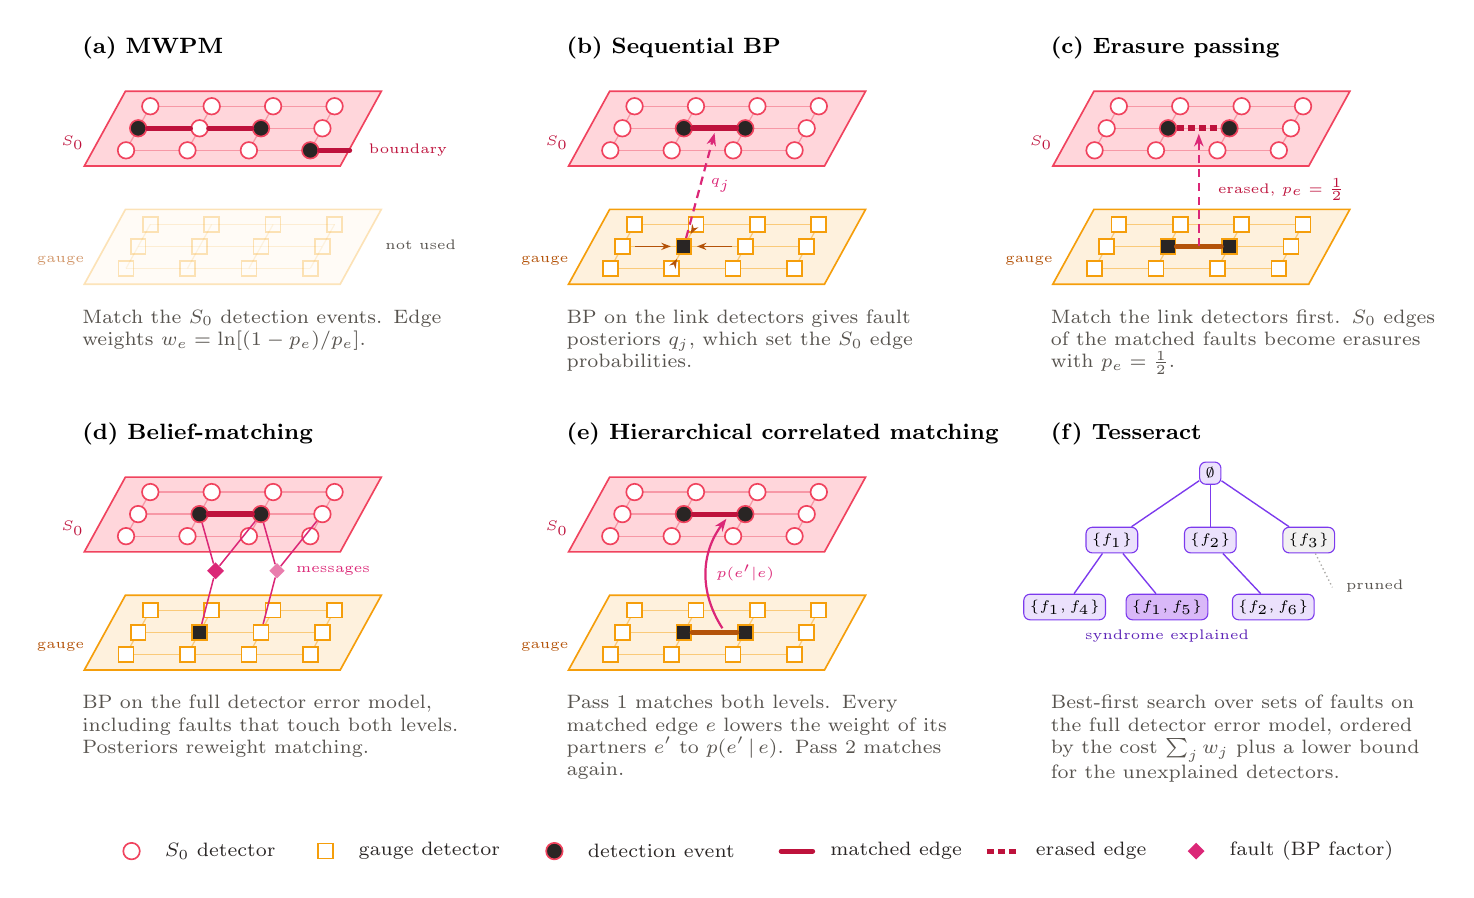
\begin{tikzpicture}
\begin{scope}[shift={(0.0,-0.0)}]
\draw[fill=Gauge!14, draw=Gauge, line width=0.6pt, opacity=0.28] (0.000,0.550) -- (3.250,0.550) -- (3.772,1.500) -- (0.522,1.500) -- cycle;
\draw[fill=ClassB!35, draw=Szero, line width=0.6pt, opacity=1.0] (0.000,2.050) -- (3.250,2.050) -- (3.772,3.000) -- (0.522,3.000) -- cycle;
\draw[line width=0.45pt, draw=Gauge!55, opacity=0.28] (0.530,0.750) -- (1.310,0.750);
\draw[line width=0.45pt, draw=Gauge!55, opacity=0.28] (0.530,0.750) -- (0.684,1.030);
\draw[line width=0.45pt, draw=Gauge!55, opacity=0.28] (0.684,1.030) -- (1.464,1.030);
\draw[line width=0.45pt, draw=Gauge!55, opacity=0.28] (0.684,1.030) -- (0.838,1.310);
\draw[line width=0.45pt, draw=Gauge!55, opacity=0.28] (0.838,1.310) -- (1.618,1.310);
\draw[line width=0.45pt, draw=Gauge!55, opacity=0.28] (1.310,0.750) -- (2.090,0.750);
\draw[line width=0.45pt, draw=Gauge!55, opacity=0.28] (1.310,0.750) -- (1.464,1.030);
\draw[line width=0.45pt, draw=Gauge!55, opacity=0.28] (1.464,1.030) -- (2.244,1.030);
\draw[line width=0.45pt, draw=Gauge!55, opacity=0.28] (1.464,1.030) -- (1.618,1.310);
\draw[line width=0.45pt, draw=Gauge!55, opacity=0.28] (1.618,1.310) -- (2.398,1.310);
\draw[line width=0.45pt, draw=Gauge!55, opacity=0.28] (2.090,0.750) -- (2.870,0.750);
\draw[line width=0.45pt, draw=Gauge!55, opacity=0.28] (2.090,0.750) -- (2.244,1.030);
\draw[line width=0.45pt, draw=Gauge!55, opacity=0.28] (2.244,1.030) -- (3.024,1.030);
\draw[line width=0.45pt, draw=Gauge!55, opacity=0.28] (2.244,1.030) -- (2.398,1.310);
\draw[line width=0.45pt, draw=Gauge!55, opacity=0.28] (2.398,1.310) -- (3.178,1.310);
\draw[line width=0.45pt, draw=Gauge!55, opacity=0.28] (2.870,0.750) -- (3.024,1.030);
\draw[line width=0.45pt, draw=Gauge!55, opacity=0.28] (3.024,1.030) -- (3.178,1.310);
\node[rectangle, minimum size=1.9mm, inner sep=0pt, draw=Gauge, line width=0.6pt, fill=white, opacity=0.28] (l00) at (0.530,0.750) {};
\node[rectangle, minimum size=1.9mm, inner sep=0pt, draw=Gauge, line width=0.6pt, fill=white, opacity=0.28] (l01) at (0.684,1.030) {};
\node[rectangle, minimum size=1.9mm, inner sep=0pt, draw=Gauge, line width=0.6pt, fill=white, opacity=0.28] (l02) at (0.838,1.310) {};
\node[rectangle, minimum size=1.9mm, inner sep=0pt, draw=Gauge, line width=0.6pt, fill=white, opacity=0.28] (l10) at (1.310,0.750) {};
\node[rectangle, minimum size=1.9mm, inner sep=0pt, draw=Gauge, line width=0.6pt, fill=white, opacity=0.28] (l11) at (1.464,1.030) {};
\node[rectangle, minimum size=1.9mm, inner sep=0pt, draw=Gauge, line width=0.6pt, fill=white, opacity=0.28] (l12) at (1.618,1.310) {};
\node[rectangle, minimum size=1.9mm, inner sep=0pt, draw=Gauge, line width=0.6pt, fill=white, opacity=0.28] (l20) at (2.090,0.750) {};
\node[rectangle, minimum size=1.9mm, inner sep=0pt, draw=Gauge, line width=0.6pt, fill=white, opacity=0.28] (l21) at (2.244,1.030) {};
\node[rectangle, minimum size=1.9mm, inner sep=0pt, draw=Gauge, line width=0.6pt, fill=white, opacity=0.28] (l22) at (2.398,1.310) {};
\node[rectangle, minimum size=1.9mm, inner sep=0pt, draw=Gauge, line width=0.6pt, fill=white, opacity=0.28] (l30) at (2.870,0.750) {};
\node[rectangle, minimum size=1.9mm, inner sep=0pt, draw=Gauge, line width=0.6pt, fill=white, opacity=0.28] (l31) at (3.024,1.030) {};
\node[rectangle, minimum size=1.9mm, inner sep=0pt, draw=Gauge, line width=0.6pt, fill=white, opacity=0.28] (l32) at (3.178,1.310) {};
\draw[line width=0.45pt, draw=Szero!55, opacity=1.0] (0.530,2.250) -- (1.310,2.250);
\draw[line width=0.45pt, draw=Szero!55, opacity=1.0] (0.530,2.250) -- (0.684,2.530);
\draw[line width=0.45pt, draw=Szero!55, opacity=1.0] (0.684,2.530) -- (1.464,2.530);
\draw[line width=0.45pt, draw=Szero!55, opacity=1.0] (0.684,2.530) -- (0.838,2.810);
\draw[line width=0.45pt, draw=Szero!55, opacity=1.0] (0.838,2.810) -- (1.618,2.810);
\draw[line width=0.45pt, draw=Szero!55, opacity=1.0] (1.310,2.250) -- (2.090,2.250);
\draw[line width=0.45pt, draw=Szero!55, opacity=1.0] (1.310,2.250) -- (1.464,2.530);
\draw[line width=0.45pt, draw=Szero!55, opacity=1.0] (1.464,2.530) -- (2.244,2.530);
\draw[line width=0.45pt, draw=Szero!55, opacity=1.0] (1.464,2.530) -- (1.618,2.810);
\draw[line width=0.45pt, draw=Szero!55, opacity=1.0] (1.618,2.810) -- (2.398,2.810);
\draw[line width=0.45pt, draw=Szero!55, opacity=1.0] (2.090,2.250) -- (2.870,2.250);
\draw[line width=0.45pt, draw=Szero!55, opacity=1.0] (2.090,2.250) -- (2.244,2.530);
\draw[line width=0.45pt, draw=Szero!55, opacity=1.0] (2.244,2.530) -- (3.024,2.530);
\draw[line width=0.45pt, draw=Szero!55, opacity=1.0] (2.244,2.530) -- (2.398,2.810);
\draw[line width=0.45pt, draw=Szero!55, opacity=1.0] (2.398,2.810) -- (3.178,2.810);
\draw[line width=0.45pt, draw=Szero!55, opacity=1.0] (2.870,2.250) -- (3.024,2.530);
\draw[line width=0.45pt, draw=Szero!55, opacity=1.0] (3.024,2.530) -- (3.178,2.810);
\node[circle, minimum size=2.1mm, inner sep=0pt, draw=Szero, line width=0.6pt, fill=white, opacity=1.0] (u00) at (0.530,2.250) {};
\node[circle, minimum size=2.1mm, inner sep=0pt, draw=Szero, line width=0.6pt, fill=InkDark, opacity=1.0] (u01) at (0.684,2.530) {};
\node[circle, minimum size=2.1mm, inner sep=0pt, draw=Szero, line width=0.6pt, fill=white, opacity=1.0] (u02) at (0.838,2.810) {};
\node[circle, minimum size=2.1mm, inner sep=0pt, draw=Szero, line width=0.6pt, fill=white, opacity=1.0] (u10) at (1.310,2.250) {};
\node[circle, minimum size=2.1mm, inner sep=0pt, draw=Szero, line width=0.6pt, fill=white, opacity=1.0] (u11) at (1.464,2.530) {};
\node[circle, minimum size=2.1mm, inner sep=0pt, draw=Szero, line width=0.6pt, fill=white, opacity=1.0] (u12) at (1.618,2.810) {};
\node[circle, minimum size=2.1mm, inner sep=0pt, draw=Szero, line width=0.6pt, fill=white, opacity=1.0] (u20) at (2.090,2.250) {};
\node[circle, minimum size=2.1mm, inner sep=0pt, draw=Szero, line width=0.6pt, fill=InkDark, opacity=1.0] (u21) at (2.244,2.530) {};
\node[circle, minimum size=2.1mm, inner sep=0pt, draw=Szero, line width=0.6pt, fill=white, opacity=1.0] (u22) at (2.398,2.810) {};
\node[circle, minimum size=2.1mm, inner sep=0pt, draw=Szero, line width=0.6pt, fill=InkDark, opacity=1.0] (u30) at (2.870,2.250) {};
\node[circle, minimum size=2.1mm, inner sep=0pt, draw=Szero, line width=0.6pt, fill=white, opacity=1.0] (u31) at (3.024,2.530) {};
\node[circle, minimum size=2.1mm, inner sep=0pt, draw=Szero, line width=0.6pt, fill=white, opacity=1.0] (u32) at (3.178,2.810) {};
\node[font=\tiny, text=SzeroText, anchor=east, opacity=1.0] at (0.12,2.35) {$S_0$};
\node[font=\tiny, text=GaugeText, anchor=east, opacity=0.6] at (0.12,0.85) {gauge};
\node[font=\footnotesize\bfseries, anchor=west] at (-0.15,3.55) {(a) MWPM};
\node[font=\scriptsize, text=InkSoft, anchor=north west, align=left, text width=4.9cm] at (-0.15,0.35) {Match the $S_0$ detection events. Edge weights $w_e=\ln[(1-p_e)/p_e]$.};
\draw[line width=1.8pt, draw=SzeroText, line cap=round] (u01) -- (u11);
\draw[line width=1.8pt, draw=SzeroText, line cap=round] (u11) -- (u21);
\draw[line width=1.8pt, draw=SzeroText, line cap=round] (u30) -- (3.370,2.250);
\node[font=\tiny, text=SzeroText, anchor=west] at (3.490,2.250) {boundary};
\node[font=\tiny, text=InkSoft, anchor=west] at (3.70,1.05) {not used};
\end{scope}
\begin{scope}[shift={(6.15,-0.0)}]
\draw[fill=Gauge!14, draw=Gauge, line width=0.6pt, opacity=1.0] (0.000,0.550) -- (3.250,0.550) -- (3.772,1.500) -- (0.522,1.500) -- cycle;
\draw[fill=ClassB!35, draw=Szero, line width=0.6pt, opacity=1.0] (0.000,2.050) -- (3.250,2.050) -- (3.772,3.000) -- (0.522,3.000) -- cycle;
\draw[line width=0.45pt, draw=Gauge!55, opacity=1.0] (0.530,0.750) -- (1.310,0.750);
\draw[line width=0.45pt, draw=Gauge!55, opacity=1.0] (0.530,0.750) -- (0.684,1.030);
\draw[line width=0.45pt, draw=Gauge!55, opacity=1.0] (0.684,1.030) -- (1.464,1.030);
\draw[line width=0.45pt, draw=Gauge!55, opacity=1.0] (0.684,1.030) -- (0.838,1.310);
\draw[line width=0.45pt, draw=Gauge!55, opacity=1.0] (0.838,1.310) -- (1.618,1.310);
\draw[line width=0.45pt, draw=Gauge!55, opacity=1.0] (1.310,0.750) -- (2.090,0.750);
\draw[line width=0.45pt, draw=Gauge!55, opacity=1.0] (1.310,0.750) -- (1.464,1.030);
\draw[line width=0.45pt, draw=Gauge!55, opacity=1.0] (1.464,1.030) -- (2.244,1.030);
\draw[line width=0.45pt, draw=Gauge!55, opacity=1.0] (1.464,1.030) -- (1.618,1.310);
\draw[line width=0.45pt, draw=Gauge!55, opacity=1.0] (1.618,1.310) -- (2.398,1.310);
\draw[line width=0.45pt, draw=Gauge!55, opacity=1.0] (2.090,0.750) -- (2.870,0.750);
\draw[line width=0.45pt, draw=Gauge!55, opacity=1.0] (2.090,0.750) -- (2.244,1.030);
\draw[line width=0.45pt, draw=Gauge!55, opacity=1.0] (2.244,1.030) -- (3.024,1.030);
\draw[line width=0.45pt, draw=Gauge!55, opacity=1.0] (2.244,1.030) -- (2.398,1.310);
\draw[line width=0.45pt, draw=Gauge!55, opacity=1.0] (2.398,1.310) -- (3.178,1.310);
\draw[line width=0.45pt, draw=Gauge!55, opacity=1.0] (2.870,0.750) -- (3.024,1.030);
\draw[line width=0.45pt, draw=Gauge!55, opacity=1.0] (3.024,1.030) -- (3.178,1.310);
\node[rectangle, minimum size=1.9mm, inner sep=0pt, draw=Gauge, line width=0.6pt, fill=white, opacity=1.0] (l00) at (0.530,0.750) {};
\node[rectangle, minimum size=1.9mm, inner sep=0pt, draw=Gauge, line width=0.6pt, fill=white, opacity=1.0] (l01) at (0.684,1.030) {};
\node[rectangle, minimum size=1.9mm, inner sep=0pt, draw=Gauge, line width=0.6pt, fill=white, opacity=1.0] (l02) at (0.838,1.310) {};
\node[rectangle, minimum size=1.9mm, inner sep=0pt, draw=Gauge, line width=0.6pt, fill=white, opacity=1.0] (l10) at (1.310,0.750) {};
\node[rectangle, minimum size=1.9mm, inner sep=0pt, draw=Gauge, line width=0.6pt, fill=InkDark, opacity=1.0] (l11) at (1.464,1.030) {};
\node[rectangle, minimum size=1.9mm, inner sep=0pt, draw=Gauge, line width=0.6pt, fill=white, opacity=1.0] (l12) at (1.618,1.310) {};
\node[rectangle, minimum size=1.9mm, inner sep=0pt, draw=Gauge, line width=0.6pt, fill=white, opacity=1.0] (l20) at (2.090,0.750) {};
\node[rectangle, minimum size=1.9mm, inner sep=0pt, draw=Gauge, line width=0.6pt, fill=white, opacity=1.0] (l21) at (2.244,1.030) {};
\node[rectangle, minimum size=1.9mm, inner sep=0pt, draw=Gauge, line width=0.6pt, fill=white, opacity=1.0] (l22) at (2.398,1.310) {};
\node[rectangle, minimum size=1.9mm, inner sep=0pt, draw=Gauge, line width=0.6pt, fill=white, opacity=1.0] (l30) at (2.870,0.750) {};
\node[rectangle, minimum size=1.9mm, inner sep=0pt, draw=Gauge, line width=0.6pt, fill=white, opacity=1.0] (l31) at (3.024,1.030) {};
\node[rectangle, minimum size=1.9mm, inner sep=0pt, draw=Gauge, line width=0.6pt, fill=white, opacity=1.0] (l32) at (3.178,1.310) {};
\draw[line width=0.45pt, draw=Szero!55, opacity=1.0] (0.530,2.250) -- (1.310,2.250);
\draw[line width=0.45pt, draw=Szero!55, opacity=1.0] (0.530,2.250) -- (0.684,2.530);
\draw[line width=0.45pt, draw=Szero!55, opacity=1.0] (0.684,2.530) -- (1.464,2.530);
\draw[line width=0.45pt, draw=Szero!55, opacity=1.0] (0.684,2.530) -- (0.838,2.810);
\draw[line width=0.45pt, draw=Szero!55, opacity=1.0] (0.838,2.810) -- (1.618,2.810);
\draw[line width=0.45pt, draw=Szero!55, opacity=1.0] (1.310,2.250) -- (2.090,2.250);
\draw[line width=0.45pt, draw=Szero!55, opacity=1.0] (1.310,2.250) -- (1.464,2.530);
\draw[line width=0.45pt, draw=Szero!55, opacity=1.0] (1.464,2.530) -- (2.244,2.530);
\draw[line width=0.45pt, draw=Szero!55, opacity=1.0] (1.464,2.530) -- (1.618,2.810);
\draw[line width=0.45pt, draw=Szero!55, opacity=1.0] (1.618,2.810) -- (2.398,2.810);
\draw[line width=0.45pt, draw=Szero!55, opacity=1.0] (2.090,2.250) -- (2.870,2.250);
\draw[line width=0.45pt, draw=Szero!55, opacity=1.0] (2.090,2.250) -- (2.244,2.530);
\draw[line width=0.45pt, draw=Szero!55, opacity=1.0] (2.244,2.530) -- (3.024,2.530);
\draw[line width=0.45pt, draw=Szero!55, opacity=1.0] (2.244,2.530) -- (2.398,2.810);
\draw[line width=0.45pt, draw=Szero!55, opacity=1.0] (2.398,2.810) -- (3.178,2.810);
\draw[line width=0.45pt, draw=Szero!55, opacity=1.0] (2.870,2.250) -- (3.024,2.530);
\draw[line width=0.45pt, draw=Szero!55, opacity=1.0] (3.024,2.530) -- (3.178,2.810);
\node[circle, minimum size=2.1mm, inner sep=0pt, draw=Szero, line width=0.6pt, fill=white, opacity=1.0] (u00) at (0.530,2.250) {};
\node[circle, minimum size=2.1mm, inner sep=0pt, draw=Szero, line width=0.6pt, fill=white, opacity=1.0] (u01) at (0.684,2.530) {};
\node[circle, minimum size=2.1mm, inner sep=0pt, draw=Szero, line width=0.6pt, fill=white, opacity=1.0] (u02) at (0.838,2.810) {};
\node[circle, minimum size=2.1mm, inner sep=0pt, draw=Szero, line width=0.6pt, fill=white, opacity=1.0] (u10) at (1.310,2.250) {};
\node[circle, minimum size=2.1mm, inner sep=0pt, draw=Szero, line width=0.6pt, fill=InkDark, opacity=1.0] (u11) at (1.464,2.530) {};
\node[circle, minimum size=2.1mm, inner sep=0pt, draw=Szero, line width=0.6pt, fill=white, opacity=1.0] (u12) at (1.618,2.810) {};
\node[circle, minimum size=2.1mm, inner sep=0pt, draw=Szero, line width=0.6pt, fill=white, opacity=1.0] (u20) at (2.090,2.250) {};
\node[circle, minimum size=2.1mm, inner sep=0pt, draw=Szero, line width=0.6pt, fill=InkDark, opacity=1.0] (u21) at (2.244,2.530) {};
\node[circle, minimum size=2.1mm, inner sep=0pt, draw=Szero, line width=0.6pt, fill=white, opacity=1.0] (u22) at (2.398,2.810) {};
\node[circle, minimum size=2.1mm, inner sep=0pt, draw=Szero, line width=0.6pt, fill=white, opacity=1.0] (u30) at (2.870,2.250) {};
\node[circle, minimum size=2.1mm, inner sep=0pt, draw=Szero, line width=0.6pt, fill=white, opacity=1.0] (u31) at (3.024,2.530) {};
\node[circle, minimum size=2.1mm, inner sep=0pt, draw=Szero, line width=0.6pt, fill=white, opacity=1.0] (u32) at (3.178,2.810) {};
\node[font=\tiny, text=SzeroText, anchor=east, opacity=1.0] at (0.12,2.35) {$S_0$};
\node[font=\tiny, text=GaugeText, anchor=east, opacity=1.0] at (0.12,0.85) {gauge};
\node[font=\footnotesize\bfseries, anchor=west] at (-0.15,3.55) {(b) Sequential BP};
\node[font=\scriptsize, text=InkSoft, anchor=north west, align=left, text width=4.9cm] at (-0.15,0.35) {BP on the link detectors gives fault posteriors $q_j$, which set the $S_0$ edge probabilities.};
\draw[-{Stealth[length=1.2mm]}, line width=0.6pt, draw=GaugeText, shorten >=0.6mm, shorten <=0.6mm] (l01) -- (l11);
\draw[-{Stealth[length=1.2mm]}, line width=0.6pt, draw=GaugeText, shorten >=0.6mm, shorten <=0.6mm] (l21) -- (l11);
\draw[-{Stealth[length=1.2mm]}, line width=0.6pt, draw=GaugeText, shorten >=0.6mm, shorten <=0.6mm] (l10) -- (l11);
\draw[-{Stealth[length=1.2mm]}, line width=0.6pt, draw=GaugeText, shorten >=0.6mm, shorten <=0.6mm] (l12) -- (l11);
\draw[-{Stealth[length=1.6mm]}, line width=0.8pt, draw=StepRec, densely dashed] (l11) -- ($(u11)!0.5!(u21)+(0,-0.06)$) node[midway, right, font=\tiny, text=StepRec] {$q_j$};
\draw[line width=2.2pt, draw=SzeroText, line cap=round] (u11) -- (u21);
\end{scope}
\begin{scope}[shift={(12.3,-0.0)}]
\draw[fill=Gauge!14, draw=Gauge, line width=0.6pt, opacity=1.0] (0.000,0.550) -- (3.250,0.550) -- (3.772,1.500) -- (0.522,1.500) -- cycle;
\draw[fill=ClassB!35, draw=Szero, line width=0.6pt, opacity=1.0] (0.000,2.050) -- (3.250,2.050) -- (3.772,3.000) -- (0.522,3.000) -- cycle;
\draw[line width=0.45pt, draw=Gauge!55, opacity=1.0] (0.530,0.750) -- (1.310,0.750);
\draw[line width=0.45pt, draw=Gauge!55, opacity=1.0] (0.530,0.750) -- (0.684,1.030);
\draw[line width=0.45pt, draw=Gauge!55, opacity=1.0] (0.684,1.030) -- (1.464,1.030);
\draw[line width=0.45pt, draw=Gauge!55, opacity=1.0] (0.684,1.030) -- (0.838,1.310);
\draw[line width=0.45pt, draw=Gauge!55, opacity=1.0] (0.838,1.310) -- (1.618,1.310);
\draw[line width=0.45pt, draw=Gauge!55, opacity=1.0] (1.310,0.750) -- (2.090,0.750);
\draw[line width=0.45pt, draw=Gauge!55, opacity=1.0] (1.310,0.750) -- (1.464,1.030);
\draw[line width=0.45pt, draw=Gauge!55, opacity=1.0] (1.464,1.030) -- (2.244,1.030);
\draw[line width=0.45pt, draw=Gauge!55, opacity=1.0] (1.464,1.030) -- (1.618,1.310);
\draw[line width=0.45pt, draw=Gauge!55, opacity=1.0] (1.618,1.310) -- (2.398,1.310);
\draw[line width=0.45pt, draw=Gauge!55, opacity=1.0] (2.090,0.750) -- (2.870,0.750);
\draw[line width=0.45pt, draw=Gauge!55, opacity=1.0] (2.090,0.750) -- (2.244,1.030);
\draw[line width=0.45pt, draw=Gauge!55, opacity=1.0] (2.244,1.030) -- (3.024,1.030);
\draw[line width=0.45pt, draw=Gauge!55, opacity=1.0] (2.244,1.030) -- (2.398,1.310);
\draw[line width=0.45pt, draw=Gauge!55, opacity=1.0] (2.398,1.310) -- (3.178,1.310);
\draw[line width=0.45pt, draw=Gauge!55, opacity=1.0] (2.870,0.750) -- (3.024,1.030);
\draw[line width=0.45pt, draw=Gauge!55, opacity=1.0] (3.024,1.030) -- (3.178,1.310);
\node[rectangle, minimum size=1.9mm, inner sep=0pt, draw=Gauge, line width=0.6pt, fill=white, opacity=1.0] (l00) at (0.530,0.750) {};
\node[rectangle, minimum size=1.9mm, inner sep=0pt, draw=Gauge, line width=0.6pt, fill=white, opacity=1.0] (l01) at (0.684,1.030) {};
\node[rectangle, minimum size=1.9mm, inner sep=0pt, draw=Gauge, line width=0.6pt, fill=white, opacity=1.0] (l02) at (0.838,1.310) {};
\node[rectangle, minimum size=1.9mm, inner sep=0pt, draw=Gauge, line width=0.6pt, fill=white, opacity=1.0] (l10) at (1.310,0.750) {};
\node[rectangle, minimum size=1.9mm, inner sep=0pt, draw=Gauge, line width=0.6pt, fill=InkDark, opacity=1.0] (l11) at (1.464,1.030) {};
\node[rectangle, minimum size=1.9mm, inner sep=0pt, draw=Gauge, line width=0.6pt, fill=white, opacity=1.0] (l12) at (1.618,1.310) {};
\node[rectangle, minimum size=1.9mm, inner sep=0pt, draw=Gauge, line width=0.6pt, fill=white, opacity=1.0] (l20) at (2.090,0.750) {};
\node[rectangle, minimum size=1.9mm, inner sep=0pt, draw=Gauge, line width=0.6pt, fill=InkDark, opacity=1.0] (l21) at (2.244,1.030) {};
\node[rectangle, minimum size=1.9mm, inner sep=0pt, draw=Gauge, line width=0.6pt, fill=white, opacity=1.0] (l22) at (2.398,1.310) {};
\node[rectangle, minimum size=1.9mm, inner sep=0pt, draw=Gauge, line width=0.6pt, fill=white, opacity=1.0] (l30) at (2.870,0.750) {};
\node[rectangle, minimum size=1.9mm, inner sep=0pt, draw=Gauge, line width=0.6pt, fill=white, opacity=1.0] (l31) at (3.024,1.030) {};
\node[rectangle, minimum size=1.9mm, inner sep=0pt, draw=Gauge, line width=0.6pt, fill=white, opacity=1.0] (l32) at (3.178,1.310) {};
\draw[line width=0.45pt, draw=Szero!55, opacity=1.0] (0.530,2.250) -- (1.310,2.250);
\draw[line width=0.45pt, draw=Szero!55, opacity=1.0] (0.530,2.250) -- (0.684,2.530);
\draw[line width=0.45pt, draw=Szero!55, opacity=1.0] (0.684,2.530) -- (1.464,2.530);
\draw[line width=0.45pt, draw=Szero!55, opacity=1.0] (0.684,2.530) -- (0.838,2.810);
\draw[line width=0.45pt, draw=Szero!55, opacity=1.0] (0.838,2.810) -- (1.618,2.810);
\draw[line width=0.45pt, draw=Szero!55, opacity=1.0] (1.310,2.250) -- (2.090,2.250);
\draw[line width=0.45pt, draw=Szero!55, opacity=1.0] (1.310,2.250) -- (1.464,2.530);
\draw[line width=0.45pt, draw=Szero!55, opacity=1.0] (1.464,2.530) -- (2.244,2.530);
\draw[line width=0.45pt, draw=Szero!55, opacity=1.0] (1.464,2.530) -- (1.618,2.810);
\draw[line width=0.45pt, draw=Szero!55, opacity=1.0] (1.618,2.810) -- (2.398,2.810);
\draw[line width=0.45pt, draw=Szero!55, opacity=1.0] (2.090,2.250) -- (2.870,2.250);
\draw[line width=0.45pt, draw=Szero!55, opacity=1.0] (2.090,2.250) -- (2.244,2.530);
\draw[line width=0.45pt, draw=Szero!55, opacity=1.0] (2.244,2.530) -- (3.024,2.530);
\draw[line width=0.45pt, draw=Szero!55, opacity=1.0] (2.244,2.530) -- (2.398,2.810);
\draw[line width=0.45pt, draw=Szero!55, opacity=1.0] (2.398,2.810) -- (3.178,2.810);
\draw[line width=0.45pt, draw=Szero!55, opacity=1.0] (2.870,2.250) -- (3.024,2.530);
\draw[line width=0.45pt, draw=Szero!55, opacity=1.0] (3.024,2.530) -- (3.178,2.810);
\node[circle, minimum size=2.1mm, inner sep=0pt, draw=Szero, line width=0.6pt, fill=white, opacity=1.0] (u00) at (0.530,2.250) {};
\node[circle, minimum size=2.1mm, inner sep=0pt, draw=Szero, line width=0.6pt, fill=white, opacity=1.0] (u01) at (0.684,2.530) {};
\node[circle, minimum size=2.1mm, inner sep=0pt, draw=Szero, line width=0.6pt, fill=white, opacity=1.0] (u02) at (0.838,2.810) {};
\node[circle, minimum size=2.1mm, inner sep=0pt, draw=Szero, line width=0.6pt, fill=white, opacity=1.0] (u10) at (1.310,2.250) {};
\node[circle, minimum size=2.1mm, inner sep=0pt, draw=Szero, line width=0.6pt, fill=InkDark, opacity=1.0] (u11) at (1.464,2.530) {};
\node[circle, minimum size=2.1mm, inner sep=0pt, draw=Szero, line width=0.6pt, fill=white, opacity=1.0] (u12) at (1.618,2.810) {};
\node[circle, minimum size=2.1mm, inner sep=0pt, draw=Szero, line width=0.6pt, fill=white, opacity=1.0] (u20) at (2.090,2.250) {};
\node[circle, minimum size=2.1mm, inner sep=0pt, draw=Szero, line width=0.6pt, fill=InkDark, opacity=1.0] (u21) at (2.244,2.530) {};
\node[circle, minimum size=2.1mm, inner sep=0pt, draw=Szero, line width=0.6pt, fill=white, opacity=1.0] (u22) at (2.398,2.810) {};
\node[circle, minimum size=2.1mm, inner sep=0pt, draw=Szero, line width=0.6pt, fill=white, opacity=1.0] (u30) at (2.870,2.250) {};
\node[circle, minimum size=2.1mm, inner sep=0pt, draw=Szero, line width=0.6pt, fill=white, opacity=1.0] (u31) at (3.024,2.530) {};
\node[circle, minimum size=2.1mm, inner sep=0pt, draw=Szero, line width=0.6pt, fill=white, opacity=1.0] (u32) at (3.178,2.810) {};
\node[font=\tiny, text=SzeroText, anchor=east, opacity=1.0] at (0.12,2.35) {$S_0$};
\node[font=\tiny, text=GaugeText, anchor=east, opacity=1.0] at (0.12,0.85) {gauge};
\node[font=\footnotesize\bfseries, anchor=west] at (-0.15,3.55) {(c) Erasure passing};
\node[font=\scriptsize, text=InkSoft, anchor=north west, align=left, text width=4.9cm] at (-0.15,0.35) {Match the link detectors first. $S_0$ edges of the matched faults become erasures with $p_e=\tfrac12$.};
\draw[line width=1.8pt, draw=GaugeText, line cap=round] (l11) -- (l21);
\draw[-{Stealth[length=1.6mm]}, line width=0.8pt, draw=StepRec, densely dashed] ($(l11)!0.5!(l21)$) -- ($(u11)!0.5!(u21)+(0,-0.07)$);
\draw[line width=2.2pt, draw=SzeroText, dash pattern=on 2.5pt off 1.5pt] (u11) -- (u21);
\node[font=\tiny, text=SzeroText, anchor=west] at ($(u11)!0.5!(u21)+(0.12,-0.78)$) {erased, $p_e=\tfrac12$};
\end{scope}
\begin{scope}[shift={(0.0,-4.9)}]
\draw[fill=Gauge!14, draw=Gauge, line width=0.6pt, opacity=1.0] (0.000,0.550) -- (3.250,0.550) -- (3.772,1.500) -- (0.522,1.500) -- cycle;
\draw[fill=ClassB!35, draw=Szero, line width=0.6pt, opacity=1.0] (0.000,2.050) -- (3.250,2.050) -- (3.772,3.000) -- (0.522,3.000) -- cycle;
\draw[line width=0.45pt, draw=Gauge!55, opacity=1.0] (0.530,0.750) -- (1.310,0.750);
\draw[line width=0.45pt, draw=Gauge!55, opacity=1.0] (0.530,0.750) -- (0.684,1.030);
\draw[line width=0.45pt, draw=Gauge!55, opacity=1.0] (0.684,1.030) -- (1.464,1.030);
\draw[line width=0.45pt, draw=Gauge!55, opacity=1.0] (0.684,1.030) -- (0.838,1.310);
\draw[line width=0.45pt, draw=Gauge!55, opacity=1.0] (0.838,1.310) -- (1.618,1.310);
\draw[line width=0.45pt, draw=Gauge!55, opacity=1.0] (1.310,0.750) -- (2.090,0.750);
\draw[line width=0.45pt, draw=Gauge!55, opacity=1.0] (1.310,0.750) -- (1.464,1.030);
\draw[line width=0.45pt, draw=Gauge!55, opacity=1.0] (1.464,1.030) -- (2.244,1.030);
\draw[line width=0.45pt, draw=Gauge!55, opacity=1.0] (1.464,1.030) -- (1.618,1.310);
\draw[line width=0.45pt, draw=Gauge!55, opacity=1.0] (1.618,1.310) -- (2.398,1.310);
\draw[line width=0.45pt, draw=Gauge!55, opacity=1.0] (2.090,0.750) -- (2.870,0.750);
\draw[line width=0.45pt, draw=Gauge!55, opacity=1.0] (2.090,0.750) -- (2.244,1.030);
\draw[line width=0.45pt, draw=Gauge!55, opacity=1.0] (2.244,1.030) -- (3.024,1.030);
\draw[line width=0.45pt, draw=Gauge!55, opacity=1.0] (2.244,1.030) -- (2.398,1.310);
\draw[line width=0.45pt, draw=Gauge!55, opacity=1.0] (2.398,1.310) -- (3.178,1.310);
\draw[line width=0.45pt, draw=Gauge!55, opacity=1.0] (2.870,0.750) -- (3.024,1.030);
\draw[line width=0.45pt, draw=Gauge!55, opacity=1.0] (3.024,1.030) -- (3.178,1.310);
\node[rectangle, minimum size=1.9mm, inner sep=0pt, draw=Gauge, line width=0.6pt, fill=white, opacity=1.0] (l00) at (0.530,0.750) {};
\node[rectangle, minimum size=1.9mm, inner sep=0pt, draw=Gauge, line width=0.6pt, fill=white, opacity=1.0] (l01) at (0.684,1.030) {};
\node[rectangle, minimum size=1.9mm, inner sep=0pt, draw=Gauge, line width=0.6pt, fill=white, opacity=1.0] (l02) at (0.838,1.310) {};
\node[rectangle, minimum size=1.9mm, inner sep=0pt, draw=Gauge, line width=0.6pt, fill=white, opacity=1.0] (l10) at (1.310,0.750) {};
\node[rectangle, minimum size=1.9mm, inner sep=0pt, draw=Gauge, line width=0.6pt, fill=InkDark, opacity=1.0] (l11) at (1.464,1.030) {};
\node[rectangle, minimum size=1.9mm, inner sep=0pt, draw=Gauge, line width=0.6pt, fill=white, opacity=1.0] (l12) at (1.618,1.310) {};
\node[rectangle, minimum size=1.9mm, inner sep=0pt, draw=Gauge, line width=0.6pt, fill=white, opacity=1.0] (l20) at (2.090,0.750) {};
\node[rectangle, minimum size=1.9mm, inner sep=0pt, draw=Gauge, line width=0.6pt, fill=white, opacity=1.0] (l21) at (2.244,1.030) {};
\node[rectangle, minimum size=1.9mm, inner sep=0pt, draw=Gauge, line width=0.6pt, fill=white, opacity=1.0] (l22) at (2.398,1.310) {};
\node[rectangle, minimum size=1.9mm, inner sep=0pt, draw=Gauge, line width=0.6pt, fill=white, opacity=1.0] (l30) at (2.870,0.750) {};
\node[rectangle, minimum size=1.9mm, inner sep=0pt, draw=Gauge, line width=0.6pt, fill=white, opacity=1.0] (l31) at (3.024,1.030) {};
\node[rectangle, minimum size=1.9mm, inner sep=0pt, draw=Gauge, line width=0.6pt, fill=white, opacity=1.0] (l32) at (3.178,1.310) {};
\draw[line width=0.45pt, draw=Szero!55, opacity=1.0] (0.530,2.250) -- (1.310,2.250);
\draw[line width=0.45pt, draw=Szero!55, opacity=1.0] (0.530,2.250) -- (0.684,2.530);
\draw[line width=0.45pt, draw=Szero!55, opacity=1.0] (0.684,2.530) -- (1.464,2.530);
\draw[line width=0.45pt, draw=Szero!55, opacity=1.0] (0.684,2.530) -- (0.838,2.810);
\draw[line width=0.45pt, draw=Szero!55, opacity=1.0] (0.838,2.810) -- (1.618,2.810);
\draw[line width=0.45pt, draw=Szero!55, opacity=1.0] (1.310,2.250) -- (2.090,2.250);
\draw[line width=0.45pt, draw=Szero!55, opacity=1.0] (1.310,2.250) -- (1.464,2.530);
\draw[line width=0.45pt, draw=Szero!55, opacity=1.0] (1.464,2.530) -- (2.244,2.530);
\draw[line width=0.45pt, draw=Szero!55, opacity=1.0] (1.464,2.530) -- (1.618,2.810);
\draw[line width=0.45pt, draw=Szero!55, opacity=1.0] (1.618,2.810) -- (2.398,2.810);
\draw[line width=0.45pt, draw=Szero!55, opacity=1.0] (2.090,2.250) -- (2.870,2.250);
\draw[line width=0.45pt, draw=Szero!55, opacity=1.0] (2.090,2.250) -- (2.244,2.530);
\draw[line width=0.45pt, draw=Szero!55, opacity=1.0] (2.244,2.530) -- (3.024,2.530);
\draw[line width=0.45pt, draw=Szero!55, opacity=1.0] (2.244,2.530) -- (2.398,2.810);
\draw[line width=0.45pt, draw=Szero!55, opacity=1.0] (2.398,2.810) -- (3.178,2.810);
\draw[line width=0.45pt, draw=Szero!55, opacity=1.0] (2.870,2.250) -- (3.024,2.530);
\draw[line width=0.45pt, draw=Szero!55, opacity=1.0] (3.024,2.530) -- (3.178,2.810);
\node[circle, minimum size=2.1mm, inner sep=0pt, draw=Szero, line width=0.6pt, fill=white, opacity=1.0] (u00) at (0.530,2.250) {};
\node[circle, minimum size=2.1mm, inner sep=0pt, draw=Szero, line width=0.6pt, fill=white, opacity=1.0] (u01) at (0.684,2.530) {};
\node[circle, minimum size=2.1mm, inner sep=0pt, draw=Szero, line width=0.6pt, fill=white, opacity=1.0] (u02) at (0.838,2.810) {};
\node[circle, minimum size=2.1mm, inner sep=0pt, draw=Szero, line width=0.6pt, fill=white, opacity=1.0] (u10) at (1.310,2.250) {};
\node[circle, minimum size=2.1mm, inner sep=0pt, draw=Szero, line width=0.6pt, fill=InkDark, opacity=1.0] (u11) at (1.464,2.530) {};
\node[circle, minimum size=2.1mm, inner sep=0pt, draw=Szero, line width=0.6pt, fill=white, opacity=1.0] (u12) at (1.618,2.810) {};
\node[circle, minimum size=2.1mm, inner sep=0pt, draw=Szero, line width=0.6pt, fill=white, opacity=1.0] (u20) at (2.090,2.250) {};
\node[circle, minimum size=2.1mm, inner sep=0pt, draw=Szero, line width=0.6pt, fill=InkDark, opacity=1.0] (u21) at (2.244,2.530) {};
\node[circle, minimum size=2.1mm, inner sep=0pt, draw=Szero, line width=0.6pt, fill=white, opacity=1.0] (u22) at (2.398,2.810) {};
\node[circle, minimum size=2.1mm, inner sep=0pt, draw=Szero, line width=0.6pt, fill=white, opacity=1.0] (u30) at (2.870,2.250) {};
\node[circle, minimum size=2.1mm, inner sep=0pt, draw=Szero, line width=0.6pt, fill=white, opacity=1.0] (u31) at (3.024,2.530) {};
\node[circle, minimum size=2.1mm, inner sep=0pt, draw=Szero, line width=0.6pt, fill=white, opacity=1.0] (u32) at (3.178,2.810) {};
\node[font=\tiny, text=SzeroText, anchor=east, opacity=1.0] at (0.12,2.35) {$S_0$};
\node[font=\tiny, text=GaugeText, anchor=east, opacity=1.0] at (0.12,0.85) {gauge};
\node[font=\footnotesize\bfseries, anchor=west] at (-0.15,3.55) {(d) Belief-matching};
\node[font=\scriptsize, text=InkSoft, anchor=north west, align=left, text width=4.9cm] at (-0.15,0.35) {BP on the full detector error model, including faults that touch both levels. Posteriors reweight matching.};
\node[diamond, fill=StepRec, minimum size=2.2mm, inner sep=0pt] (fa) at ($($(u11)!0.5!(u21)$)!0.48!(l11)$) {};
\node[diamond, fill=StepRec!60, minimum size=2.0mm, inner sep=0pt] (fb) at ($($(u21)!0.5!(u31)$)!0.48!(l21)$) {};
\draw[line width=0.55pt, draw=StepRec] (fa) -- (u11);
\draw[line width=0.55pt, draw=StepRec] (fa) -- (u21);
\draw[line width=0.55pt, draw=StepRec] (fa) -- (l11);
\draw[line width=0.55pt, draw=StepRec] (fb) -- (u21);
\draw[line width=0.55pt, draw=StepRec] (fb) -- (u31);
\draw[line width=0.55pt, draw=StepRec] (fb) -- (l21);
\draw[line width=2.2pt, draw=SzeroText, line cap=round] (u11) -- (u21);
\node[font=\tiny, text=StepRec, anchor=west] at ($(fb)+(0.12,0.0)$) {messages};
\end{scope}
\begin{scope}[shift={(6.15,-4.9)}]
\draw[fill=Gauge!14, draw=Gauge, line width=0.6pt, opacity=1.0] (0.000,0.550) -- (3.250,0.550) -- (3.772,1.500) -- (0.522,1.500) -- cycle;
\draw[fill=ClassB!35, draw=Szero, line width=0.6pt, opacity=1.0] (0.000,2.050) -- (3.250,2.050) -- (3.772,3.000) -- (0.522,3.000) -- cycle;
\draw[line width=0.45pt, draw=Gauge!55, opacity=1.0] (0.530,0.750) -- (1.310,0.750);
\draw[line width=0.45pt, draw=Gauge!55, opacity=1.0] (0.530,0.750) -- (0.684,1.030);
\draw[line width=0.45pt, draw=Gauge!55, opacity=1.0] (0.684,1.030) -- (1.464,1.030);
\draw[line width=0.45pt, draw=Gauge!55, opacity=1.0] (0.684,1.030) -- (0.838,1.310);
\draw[line width=0.45pt, draw=Gauge!55, opacity=1.0] (0.838,1.310) -- (1.618,1.310);
\draw[line width=0.45pt, draw=Gauge!55, opacity=1.0] (1.310,0.750) -- (2.090,0.750);
\draw[line width=0.45pt, draw=Gauge!55, opacity=1.0] (1.310,0.750) -- (1.464,1.030);
\draw[line width=0.45pt, draw=Gauge!55, opacity=1.0] (1.464,1.030) -- (2.244,1.030);
\draw[line width=0.45pt, draw=Gauge!55, opacity=1.0] (1.464,1.030) -- (1.618,1.310);
\draw[line width=0.45pt, draw=Gauge!55, opacity=1.0] (1.618,1.310) -- (2.398,1.310);
\draw[line width=0.45pt, draw=Gauge!55, opacity=1.0] (2.090,0.750) -- (2.870,0.750);
\draw[line width=0.45pt, draw=Gauge!55, opacity=1.0] (2.090,0.750) -- (2.244,1.030);
\draw[line width=0.45pt, draw=Gauge!55, opacity=1.0] (2.244,1.030) -- (3.024,1.030);
\draw[line width=0.45pt, draw=Gauge!55, opacity=1.0] (2.244,1.030) -- (2.398,1.310);
\draw[line width=0.45pt, draw=Gauge!55, opacity=1.0] (2.398,1.310) -- (3.178,1.310);
\draw[line width=0.45pt, draw=Gauge!55, opacity=1.0] (2.870,0.750) -- (3.024,1.030);
\draw[line width=0.45pt, draw=Gauge!55, opacity=1.0] (3.024,1.030) -- (3.178,1.310);
\node[rectangle, minimum size=1.9mm, inner sep=0pt, draw=Gauge, line width=0.6pt, fill=white, opacity=1.0] (l00) at (0.530,0.750) {};
\node[rectangle, minimum size=1.9mm, inner sep=0pt, draw=Gauge, line width=0.6pt, fill=white, opacity=1.0] (l01) at (0.684,1.030) {};
\node[rectangle, minimum size=1.9mm, inner sep=0pt, draw=Gauge, line width=0.6pt, fill=white, opacity=1.0] (l02) at (0.838,1.310) {};
\node[rectangle, minimum size=1.9mm, inner sep=0pt, draw=Gauge, line width=0.6pt, fill=white, opacity=1.0] (l10) at (1.310,0.750) {};
\node[rectangle, minimum size=1.9mm, inner sep=0pt, draw=Gauge, line width=0.6pt, fill=InkDark, opacity=1.0] (l11) at (1.464,1.030) {};
\node[rectangle, minimum size=1.9mm, inner sep=0pt, draw=Gauge, line width=0.6pt, fill=white, opacity=1.0] (l12) at (1.618,1.310) {};
\node[rectangle, minimum size=1.9mm, inner sep=0pt, draw=Gauge, line width=0.6pt, fill=white, opacity=1.0] (l20) at (2.090,0.750) {};
\node[rectangle, minimum size=1.9mm, inner sep=0pt, draw=Gauge, line width=0.6pt, fill=InkDark, opacity=1.0] (l21) at (2.244,1.030) {};
\node[rectangle, minimum size=1.9mm, inner sep=0pt, draw=Gauge, line width=0.6pt, fill=white, opacity=1.0] (l22) at (2.398,1.310) {};
\node[rectangle, minimum size=1.9mm, inner sep=0pt, draw=Gauge, line width=0.6pt, fill=white, opacity=1.0] (l30) at (2.870,0.750) {};
\node[rectangle, minimum size=1.9mm, inner sep=0pt, draw=Gauge, line width=0.6pt, fill=white, opacity=1.0] (l31) at (3.024,1.030) {};
\node[rectangle, minimum size=1.9mm, inner sep=0pt, draw=Gauge, line width=0.6pt, fill=white, opacity=1.0] (l32) at (3.178,1.310) {};
\draw[line width=0.45pt, draw=Szero!55, opacity=1.0] (0.530,2.250) -- (1.310,2.250);
\draw[line width=0.45pt, draw=Szero!55, opacity=1.0] (0.530,2.250) -- (0.684,2.530);
\draw[line width=0.45pt, draw=Szero!55, opacity=1.0] (0.684,2.530) -- (1.464,2.530);
\draw[line width=0.45pt, draw=Szero!55, opacity=1.0] (0.684,2.530) -- (0.838,2.810);
\draw[line width=0.45pt, draw=Szero!55, opacity=1.0] (0.838,2.810) -- (1.618,2.810);
\draw[line width=0.45pt, draw=Szero!55, opacity=1.0] (1.310,2.250) -- (2.090,2.250);
\draw[line width=0.45pt, draw=Szero!55, opacity=1.0] (1.310,2.250) -- (1.464,2.530);
\draw[line width=0.45pt, draw=Szero!55, opacity=1.0] (1.464,2.530) -- (2.244,2.530);
\draw[line width=0.45pt, draw=Szero!55, opacity=1.0] (1.464,2.530) -- (1.618,2.810);
\draw[line width=0.45pt, draw=Szero!55, opacity=1.0] (1.618,2.810) -- (2.398,2.810);
\draw[line width=0.45pt, draw=Szero!55, opacity=1.0] (2.090,2.250) -- (2.870,2.250);
\draw[line width=0.45pt, draw=Szero!55, opacity=1.0] (2.090,2.250) -- (2.244,2.530);
\draw[line width=0.45pt, draw=Szero!55, opacity=1.0] (2.244,2.530) -- (3.024,2.530);
\draw[line width=0.45pt, draw=Szero!55, opacity=1.0] (2.244,2.530) -- (2.398,2.810);
\draw[line width=0.45pt, draw=Szero!55, opacity=1.0] (2.398,2.810) -- (3.178,2.810);
\draw[line width=0.45pt, draw=Szero!55, opacity=1.0] (2.870,2.250) -- (3.024,2.530);
\draw[line width=0.45pt, draw=Szero!55, opacity=1.0] (3.024,2.530) -- (3.178,2.810);
\node[circle, minimum size=2.1mm, inner sep=0pt, draw=Szero, line width=0.6pt, fill=white, opacity=1.0] (u00) at (0.530,2.250) {};
\node[circle, minimum size=2.1mm, inner sep=0pt, draw=Szero, line width=0.6pt, fill=white, opacity=1.0] (u01) at (0.684,2.530) {};
\node[circle, minimum size=2.1mm, inner sep=0pt, draw=Szero, line width=0.6pt, fill=white, opacity=1.0] (u02) at (0.838,2.810) {};
\node[circle, minimum size=2.1mm, inner sep=0pt, draw=Szero, line width=0.6pt, fill=white, opacity=1.0] (u10) at (1.310,2.250) {};
\node[circle, minimum size=2.1mm, inner sep=0pt, draw=Szero, line width=0.6pt, fill=InkDark, opacity=1.0] (u11) at (1.464,2.530) {};
\node[circle, minimum size=2.1mm, inner sep=0pt, draw=Szero, line width=0.6pt, fill=white, opacity=1.0] (u12) at (1.618,2.810) {};
\node[circle, minimum size=2.1mm, inner sep=0pt, draw=Szero, line width=0.6pt, fill=white, opacity=1.0] (u20) at (2.090,2.250) {};
\node[circle, minimum size=2.1mm, inner sep=0pt, draw=Szero, line width=0.6pt, fill=InkDark, opacity=1.0] (u21) at (2.244,2.530) {};
\node[circle, minimum size=2.1mm, inner sep=0pt, draw=Szero, line width=0.6pt, fill=white, opacity=1.0] (u22) at (2.398,2.810) {};
\node[circle, minimum size=2.1mm, inner sep=0pt, draw=Szero, line width=0.6pt, fill=white, opacity=1.0] (u30) at (2.870,2.250) {};
\node[circle, minimum size=2.1mm, inner sep=0pt, draw=Szero, line width=0.6pt, fill=white, opacity=1.0] (u31) at (3.024,2.530) {};
\node[circle, minimum size=2.1mm, inner sep=0pt, draw=Szero, line width=0.6pt, fill=white, opacity=1.0] (u32) at (3.178,2.810) {};
\node[font=\tiny, text=SzeroText, anchor=east, opacity=1.0] at (0.12,2.35) {$S_0$};
\node[font=\tiny, text=GaugeText, anchor=east, opacity=1.0] at (0.12,0.85) {gauge};
\node[font=\footnotesize\bfseries, anchor=west] at (-0.15,3.55) {(e) Hierarchical correlated matching};
\node[font=\scriptsize, text=InkSoft, anchor=north west, align=left, text width=4.9cm] at (-0.15,0.35) {Pass 1 matches both levels. Every matched edge $e$ lowers the weight of its partners $e'$ to $p(e'\,|\,e)$. Pass 2 matches again.};
\draw[line width=1.8pt, draw=GaugeText, line cap=round] (l11) -- (l21);
\draw[line width=1.8pt, draw=SzeroText, line cap=round] (u11) -- (u21);
\draw[-{Stealth[length=1.6mm]}, line width=0.8pt, draw=StepRec, bend left=35] ($(l11)!0.5!(l21)+(0.1,0.05)$) to node[right, font=\tiny, text=StepRec] {$p(e'|e)$} ($(u11)!0.5!(u21)+(0.15,-0.06)$);
\end{scope}
\begin{scope}[shift={(12.3,-4.9)}]
\node[font=\footnotesize\bfseries, anchor=west] at (-0.15,3.55) {(f) Tesseract};
\node[draw=StepDec, fill=StepDec!15, rounded corners=0.8mm, font=\tiny, inner sep=2pt] (r) at (2.0,3.05) {$\emptyset$};
\node[draw=StepDec, fill=StepDec!15, rounded corners=0.8mm, font=\tiny, inner sep=2pt] (k1) at (0.75,2.2) {$\{f_1\}$};
\draw[line width=0.5pt, draw=StepDec] (r) -- (k1);
\node[draw=StepDec, fill=StepDec!15, rounded corners=0.8mm, font=\tiny, inner sep=2pt] (k2) at (2.0,2.2) {$\{f_2\}$};
\draw[line width=0.5pt, draw=StepDec] (r) -- (k2);
\node[draw=StepDec, fill=InkSoft!8, rounded corners=0.8mm, font=\tiny, inner sep=2pt] (k3) at (3.25,2.2) {$\{f_3\}$};
\draw[line width=0.5pt, draw=StepDec] (r) -- (k3);
\node[draw=StepDec, fill=StepDec!15, rounded corners=0.8mm, font=\tiny, inner sep=2pt] (g1) at (0.15,1.35) {$\{f_1,f_4\}$};
\node[draw=StepDec, fill=PauliZ!35, rounded corners=0.8mm, font=\tiny, inner sep=2pt] (g2) at (1.45,1.35) {$\{f_1,f_5\}$};
\node[draw=StepDec, fill=StepDec!15, rounded corners=0.8mm, font=\tiny, inner sep=2pt] (g3) at (2.8,1.35) {$\{f_2,f_6\}$};
\draw[line width=0.5pt, draw=StepDec] (k1) -- (g1); \draw[line width=0.5pt, draw=StepDec] (k1) -- (g2); \draw[line width=0.5pt, draw=StepDec] (k2) -- (g3);
\draw[line width=0.5pt, draw=InkSoft!50, densely dotted] (k3) -- +(0.3,-0.6);
\node[font=\tiny, text=PauliZText, anchor=north] at (g2.south) {syndrome explained};
\node[font=\tiny, text=InkSoft, anchor=west] at (3.6,1.62) {pruned};
\node[font=\scriptsize, text=InkSoft, anchor=north west, align=left, text width=4.9cm] at (-0.15,0.35) {Best-first search over sets of faults on the full detector error model, ordered by the cost $\sum_j w_j$ plus a lower bound for the unexplained detectors.};
\end{scope}
\begin{scope}
\begin{scope}[shift={(0.60,0)}]\node[circle, minimum size=2.1mm, inner sep=0pt, draw=Szero, line width=0.6pt, fill=white] at (0,-6.65) {};\node[font=\scriptsize, anchor=west, text=InkDark] at (0.3,-6.65) {$S_0$ detector};\end{scope}
\begin{scope}[shift={(3.06,0)}]\node[rectangle, minimum size=1.9mm, inner sep=0pt, draw=Gauge, line width=0.6pt, fill=white] at (0,-6.65) {};\node[font=\scriptsize, anchor=west, text=InkDark] at (0.3,-6.65) {gauge detector};\end{scope}
\begin{scope}[shift={(5.97,0)}]\node[circle, minimum size=2.1mm, inner sep=0pt, draw=Szero, line width=0.6pt, fill=InkDark] at (0,-6.65) {};\node[font=\scriptsize, anchor=west, text=InkDark] at (0.3,-6.65) {detection event};\end{scope}
\begin{scope}[shift={(9.05,0)}]\draw[line width=1.8pt, draw=SzeroText, line cap=round] (-0.2,-6.65) -- (0.2,-6.65);\node[font=\scriptsize, anchor=west, text=InkDark] at (0.3,-6.65) {matched edge};\end{scope}
\begin{scope}[shift={(11.66,0)}]\draw[line width=1.8pt, draw=SzeroText, dash pattern=on 2.5pt off 1.5pt] (-0.2,-6.65) -- (0.2,-6.65);\node[font=\scriptsize, anchor=west, text=InkDark] at (0.3,-6.65) {erased edge};\end{scope}
\begin{scope}[shift={(14.12,0)}]\node[diamond, fill=StepRec, minimum size=2.2mm, inner sep=0pt] at (0,-6.65) {};\node[font=\scriptsize, anchor=west, text=InkDark] at (0.3,-6.65) {fault (BP factor)};\end{scope}
\end{scope}
\end{tikzpicture}

\end{document}
